%Version 3.1 December 2024
% See section 11 of the User Manual for version history
%
%%%%%%%%%%%%%%%%%%%%%%%%%%%%%%%%%%%%%%%%%%%%%%%%%%%%%%%%%%%%%%%%%%%%%%
%%                                                                 %%
%% Please do not use \input{...} to include other tex files.       %%
%% Submit your LaTeX manuscript as one .tex document.              %%
%%                                                                 %%
%% All additional figures and files should be attached             %%
%% separately and not embedded in the \TeX\ document itself.       %%
%%                                                                 %%
%%%%%%%%%%%%%%%%%%%%%%%%%%%%%%%%%%%%%%%%%%%%%%%%%%%%%%%%%%%%%%%%%%%%%

%%\documentclass[referee,sn-basic]{sn-jnl}% referee option is meant for double line spacing

%%=======================================================%%
%% to print line numbers in the margin use lineno option %%
%%=======================================================%%

\documentclass[lineno,pdflatex,sn-basic]{sn-jnl}% Basic Springer Nature Reference Style/Chemistry Reference Style

%%=========================================================================================%%
%% the documentclass is set to pdflatex as default. You can delete it if not appropriate.  %%
%%=========================================================================================%%

%%\documentclass[sn-basic]{sn-jnl}% Basic Springer Nature Reference Style/Chemistry Reference Style

%%Note: the following reference styles support Namedate and Numbered referencing. By default the style follows the most common style. To switch between the options you can add or remove �Numbered� in the optional parenthesis. 
%%The option is available for: sn-basic.bst, sn-chicago.bst%  
 
%%\documentclass[pdflatex,sn-nature]{sn-jnl}% Style for submissions to Nature Portfolio journals
%%\documentclass[pdflatex,sn-basic]{sn-jnl}% Basic Springer Nature Reference Style/Chemistry Reference Style
% \documentclass[pdflatex,sn-mathphys-num]{sn-jnl}% Math and Physical Sciences Numbered Reference Style
%%\documentclass[pdflatex,sn-mathphys-ay]{sn-jnl}% Math and Physical Sciences Author Year Reference Style
%%\documentclass[pdflatex,sn-aps]{sn-jnl}% American Physical Society (APS) Reference Style
%%\documentclass[pdflatex,sn-vancouver-num]{sn-jnl}% Vancouver Numbered Reference Style
%%\documentclass[pdflatex,sn-vancouver-ay]{sn-jnl}% Vancouver Author Year Reference Style
%%\documentclass[pdflatex,sn-apa]{sn-jnl}% APA Reference Style
%%\documentclass[pdflatex,sn-chicago]{sn-jnl}% Chicago-based Humanities Reference Style

%%%% Standard Packages
%%<additional latex packages if required can be included here>

\usepackage{graphicx}%
\usepackage{multirow}%
\usepackage{amsmath,amssymb,amsfonts}%
\usepackage{amsthm}%
\usepackage{mathrsfs}%
\usepackage[title]{appendix}%
\usepackage{xcolor}%
\usepackage{textcomp}%
\usepackage{manyfoot}%
\usepackage{booktabs}%
\usepackage{algorithm}%
\usepackage{algorithmicx}%
\usepackage{algpseudocode}%
\usepackage{listings}%
%%%%

%%%%%=============================================================================%%%%
%%%%  Remarks: This template is provided to aid authors with the preparation
%%%%  of original research articles intended for submission to journals published 
%%%%  by Springer Nature. The guidance has been prepared in partnership with 
%%%%  production teams to conform to Springer Nature technical requirements. 
%%%%  Editorial and presentation requirements differ among journal portfolios and 
%%%%  research disciplines. You may find sections in this template are irrelevant 
%%%%  to your work and are empowered to omit any such section if allowed by the 
%%%%  journal you intend to submit to. The submission guidelines and policies 
%%%%  of the journal take precedence. A detailed User Manual is available in the 
%%%%  template package for technical guidance.
%%%%%=============================================================================%%%%

%% as per the requirement new theorem styles can be included as shown below
\theoremstyle{thmstyleone}%
\newtheorem{theorem}{Theorem}%  meant for continuous numbers
%%\newtheorem{theorem}{Theorem}[section]% meant for sectionwise numbers
%% optional argument [theorem] produces theorem numbering sequence instead of independent numbers for Proposition
\newtheorem{proposition}[theorem]{Proposition}% 
%%\newtheorem{proposition}{Proposition}% to get separate numbers for theorem and proposition etc.

\theoremstyle{thmstyletwo}%
\newtheorem{example}{Example}%
\newtheorem{remark}{Remark}%

\theoremstyle{thmstylethree}%
\newtheorem{definition}{Definition}%

\raggedbottom
%%\unnumbered% uncomment this for unnumbered level heads

% Generated from selected result files.
\newcommand{\ScenarioCount}{30}
\newcommand{\ValidatedScriptCount}{0}
\newcommand{\EOneResources}{1,347}
\newcommand{\EOneErrors}{0}
\newcommand{\EOneWarnings}{1,750}
\newcommand{\EOneValidatorCrashes}{0}
\newcommand{\EOneTemplatedSessions}{200}
\newcommand{\EOneScenarioSessions}{150}
\newcommand{\ETwoSessions}{150}
\newcommand{\ETwoRepeats}{5}
\newcommand{\EThreeConfigurations}{3}
\newcommand{\EThreeHandoffs}{2}
\newcommand{\InputBundles}{1,000}
\newcommand{\InputResources}{430,017}
\newcommand{\InputErrors}{0}
\newcommand{\InputWarnings}{1,058,802}
\newcommand{\ELoadLastConcurrency}{500}
\newcommand{\ELoadLastCompleted}{130}
\newcommand{\ELoadLastSessions}{500}
\newcommand{\ERealSessions}{7}
\newcommand{\ERealCompleted}{7}
\newcommand{\EOneQuestionnaireResponses}{350}
\newcommand{\EOneQRWithErrors}{0}
\newcommand{\EOneQRErrors}{0}
\newcommand{\EOneQRUnverified}{0}
\newcommand{\EOneQRVerified}{350}
\newcommand{\EOneProvenanceWarnings}{1,400}
\newcommand{\EOneCompositionWarnings}{350}
\newcommand{\ETwoFacts}{454}
\newcommand{\ETwoCompleted}{150}
\newcommand{\ETwoChiefStops}{50}
\newcommand{\ETwoChiefStopsCompleted}{50}
\newcommand{\ETwoUnexpectedStops}{0}
\newcommand{\ETwoHandoffs}{0}
\newcommand{\ETwoInvalidTurns}{48}
\newcommand{\ETwoProtocolExcluded}{50}
\newcommand{\ETwoUsageCalls}{1,381}
\newcommand{\ETwoUsageEmptySessions}{40}
\newcommand{\ETwoUsageIncompleteSessions}{150}
\newcommand{\ETwoCostSessions}{110}
\newcommand{\ETwoTimeoutSessions}{1}
\newcommand{\ETwoTimeoutStored}{1}
\newcommand{\ETwoTimeoutWriteback}{1}
\newcommand{\ETwoTimeoutCompleted}{1}
\newcommand{\ETwoTimeoutFreeCompleted}{149}
\newcommand{\ETwoTimeoutEvents}{1}
\newcommand{\ETwoTimeoutLogEvents}{1}
\newcommand{\ETwoSchemaFailures}{0}
\newcommand{\ETwoChiefCalls}{110}
\newcommand{\ETwoParsedEmptyCalls}{0}
\newcommand{\ETwoGroundingFailedChecks}{17,689}
\newcommand{\ETwoParsedSymptoms}{110}
\newcommand{\ETwoRetainedSymptoms}{110}
\newcommand{\ETwoParsedFindings}{262}
\newcommand{\ETwoRetainedFindings}{262}
\newcommand{\ETwoParsedAssessments}{110}
\newcommand{\ETwoRetainedAssessments}{110}
\newcommand{\ETwoParsedAnswers}{232}
\newcommand{\ETwoRetainedAnswers}{267}
\newcommand{\ETwoCompletion}{100.0\% (150/150)}
\newcommand{\ETwoProtocol}{100.0\% (100/100)}
\newcommand{\ETwoFunctionalPass}{83.3\% (50/60)}
\newcommand{\ETwoNonRedFunctionalPass}{100.0\% (90/90)}
\newcommand{\ETwoMedianSeconds}{34.6}
\newcommand{\ETwoMedianCost}{0.0177}
\newcommand{\EThreeDefaultSessions}{30}
\newcommand{\EThreeDefaultFacts}{91}
\newcommand{\EThreeDefaultCompleted}{30}
\newcommand{\EThreeDefaultChiefStops}{10}
\newcommand{\EThreeDefaultChiefStopsCompleted}{10}
\newcommand{\EThreeDefaultUnexpectedStops}{0}
\newcommand{\EThreeDefaultHandoffs}{0}
\newcommand{\EThreeDefaultInvalidTurns}{10}
\newcommand{\EThreeDefaultProtocolExcluded}{10}
\newcommand{\EThreeDefaultUsageCalls}{322}
\newcommand{\EThreeDefaultUsageEmptySessions}{8}
\newcommand{\EThreeDefaultUsageIncompleteSessions}{30}
\newcommand{\EThreeDefaultCostSessions}{22}
\newcommand{\EThreeDefaultTimeoutSessions}{0}
\newcommand{\EThreeDefaultTimeoutStored}{0}
\newcommand{\EThreeDefaultTimeoutWriteback}{0}
\newcommand{\EThreeDefaultTimeoutCompleted}{0}
\newcommand{\EThreeDefaultTimeoutFreeCompleted}{30}
\newcommand{\EThreeDefaultTimeoutEvents}{0}
\newcommand{\EThreeDefaultTimeoutLogEvents}{0}
\newcommand{\EThreeDefaultSchemaFailures}{0}
\newcommand{\EThreeDefaultChiefCalls}{22}
\newcommand{\EThreeDefaultParsedEmptyCalls}{0}
\newcommand{\EThreeDefaultGroundingFailedChecks}{3,539}
\newcommand{\EThreeDefaultParsedSymptoms}{22}
\newcommand{\EThreeDefaultRetainedSymptoms}{22}
\newcommand{\EThreeDefaultParsedFindings}{52}
\newcommand{\EThreeDefaultRetainedFindings}{51}
\newcommand{\EThreeDefaultParsedAssessments}{22}
\newcommand{\EThreeDefaultRetainedAssessments}{22}
\newcommand{\EThreeDefaultParsedAnswers}{45}
\newcommand{\EThreeDefaultRetainedAnswers}{52}
\newcommand{\EThreeDefaultCompletion}{100.0\% (30/30)}
\newcommand{\EThreeDefaultProtocol}{100.0\% (20/20)}
\newcommand{\EThreeDefaultFunctionalPass}{83.3\% (10/12)}
\newcommand{\EThreeDefaultNonRedFunctionalPass}{100.0\% (18/18)}
\newcommand{\EThreeDefaultMedianSeconds}{40.0}
\newcommand{\EThreeDefaultMedianCost}{0.0192}
\newcommand{\EThreeAlternateSessions}{30}
\newcommand{\EThreeAlternateFacts}{114}
\newcommand{\EThreeAlternateCompleted}{30}
\newcommand{\EThreeAlternateChiefStops}{10}
\newcommand{\EThreeAlternateChiefStopsCompleted}{10}
\newcommand{\EThreeAlternateUnexpectedStops}{0}
\newcommand{\EThreeAlternateHandoffs}{0}
\newcommand{\EThreeAlternateInvalidTurns}{10}
\newcommand{\EThreeAlternateProtocolExcluded}{10}
\newcommand{\EThreeAlternateUsageCalls}{321}
\newcommand{\EThreeAlternateUsageEmptySessions}{8}
\newcommand{\EThreeAlternateUsageIncompleteSessions}{30}
\newcommand{\EThreeAlternateCostSessions}{22}
\newcommand{\EThreeAlternateTimeoutSessions}{2}
\newcommand{\EThreeAlternateTimeoutStored}{2}
\newcommand{\EThreeAlternateTimeoutWriteback}{2}
\newcommand{\EThreeAlternateTimeoutCompleted}{2}
\newcommand{\EThreeAlternateTimeoutFreeCompleted}{28}
\newcommand{\EThreeAlternateTimeoutEvents}{2}
\newcommand{\EThreeAlternateTimeoutLogEvents}{2}
\newcommand{\EThreeAlternateSchemaFailures}{0}
\newcommand{\EThreeAlternateChiefCalls}{22}
\newcommand{\EThreeAlternateParsedEmptyCalls}{0}
\newcommand{\EThreeAlternateGroundingFailedChecks}{3,540}
\newcommand{\EThreeAlternateParsedSymptoms}{28}
\newcommand{\EThreeAlternateRetainedSymptoms}{22}
\newcommand{\EThreeAlternateParsedFindings}{53}
\newcommand{\EThreeAlternateRetainedFindings}{53}
\newcommand{\EThreeAlternateParsedAssessments}{28}
\newcommand{\EThreeAlternateRetainedAssessments}{22}
\newcommand{\EThreeAlternateParsedAnswers}{67}
\newcommand{\EThreeAlternateRetainedAnswers}{70}
\newcommand{\EThreeAlternateCompletion}{100.0\% (30/30)}
\newcommand{\EThreeAlternateProtocol}{100.0\% (20/20)}
\newcommand{\EThreeAlternateFunctionalPass}{83.3\% (10/12)}
\newcommand{\EThreeAlternateNonRedFunctionalPass}{100.0\% (18/18)}
\newcommand{\EThreeAlternateMedianSeconds}{34.5}
\newcommand{\EThreeAlternateMedianCost}{0.0096}
\newcommand{\EThreeLocalSessions}{30}
\newcommand{\EThreeLocalFacts}{6}
\newcommand{\EThreeLocalCompleted}{28}
\newcommand{\EThreeLocalChiefStops}{10}
\newcommand{\EThreeLocalChiefStopsCompleted}{8}
\newcommand{\EThreeLocalUnexpectedStops}{2}
\newcommand{\EThreeLocalHandoffs}{2}
\newcommand{\EThreeLocalInvalidTurns}{10}
\newcommand{\EThreeLocalProtocolExcluded}{8}
\newcommand{\EThreeLocalUsageCalls}{311}
\newcommand{\EThreeLocalUsageEmptySessions}{10}
\newcommand{\EThreeLocalUsageIncompleteSessions}{30}
\newcommand{\EThreeLocalCostSessions}{20}
\newcommand{\EThreeLocalTimeoutSessions}{12}
\newcommand{\EThreeLocalTimeoutStored}{12}
\newcommand{\EThreeLocalTimeoutWriteback}{12}
\newcommand{\EThreeLocalTimeoutCompleted}{10}
\newcommand{\EThreeLocalTimeoutFreeCompleted}{18}
\newcommand{\EThreeLocalTimeoutEvents}{12}
\newcommand{\EThreeLocalTimeoutLogEvents}{10}
\newcommand{\EThreeLocalSchemaFailures}{0}
\newcommand{\EThreeLocalChiefCalls}{22}
\newcommand{\EThreeLocalParsedEmptyCalls}{0}
\newcommand{\EThreeLocalGroundingFailedChecks}{3,634}
\newcommand{\EThreeLocalParsedSymptoms}{108}
\newcommand{\EThreeLocalRetainedSymptoms}{6}
\newcommand{\EThreeLocalParsedFindings}{0}
\newcommand{\EThreeLocalRetainedFindings}{0}
\newcommand{\EThreeLocalParsedAssessments}{22}
\newcommand{\EThreeLocalRetainedAssessments}{0}
\newcommand{\EThreeLocalParsedAnswers}{0}
\newcommand{\EThreeLocalRetainedAnswers}{20}
\newcommand{\EThreeLocalCompletion}{93.3\% (28/30)}
\newcommand{\EThreeLocalProtocol}{90.9\% (20/22)}
\newcommand{\EThreeLocalFunctionalPass}{66.7\% (8/12)}
\newcommand{\EThreeLocalNonRedFunctionalPass}{100.0\% (18/18)}
\newcommand{\EThreeLocalMedianSeconds}{205.7}
\newcommand{\EThreeLocalMedianCost}{0.0000}
\newcommand{\AdapterAdded}{682}
\newcommand{\AdapterRemoved}{60}
\newcommand{\ELoadHundredPninetyfiveSeconds}{121.3}
\newcommand{\ELoadHundredConcurrency}{100}
\newcommand{\ETwoTraceability}{100.0\% (454/454)}
\newcommand{\ELoadLastRequestError}{4.71\%}
\newcommand{\ELoadLastSessionFailure}{74.0\%}
\newcommand{\ERealConcurrency}{1, 2, 4}
\newcommand{\ResultsStatus}{Provisional; physician scenario review pending}

\begin{document}

\title[FHIR-integrated pre-consultation]{A Modular, FHIR-Integrated Framework for LLM-Assisted Pre-Consultation}

%%=============================================================%%
%% GivenName	-> \fnm{Joergen W.}
%% Particle	-> \spfx{van der} -> surname prefix
%% FamilyName	-> \sur{Ploeg}
%% Suffix	-> \sfx{IV}
%% \author*[1,2]{\fnm{Joergen W.} \spfx{van der} \sur{Ploeg} 
%%  \sfx{IV}}\email{iauthor@gmail.com}
%%=============================================================%%

\author[1,2,3]{\fnm{Wei-Hsuan} \sur{Tai}}\email{b12508026@ntu.edu.tw}\equalcont{These authors contributed equally to this work.}


\author[2,3]{\fnm{Chun-Yi} \sur{Chen}}\email{TODO}\equalcont{These authors contributed equally to this work.}


\author[4]{\fnm{Guan-Ying} \sur{Huang}}\email{TODO}\equalcont{These authors contributed equally to this work.}


\author*[4,5,6]{\fnm{Chien-Chang} \sur{Lee}}\email{cclee100@gmail.com}

\affil[1]{\orgdiv{Department of Biomedical Engineering}, \orgname{National Taiwan University}, \orgaddress{\city{Taipei}, \country{Taiwan}}}

% TODO: confirm ISTI's official English name and city (Hsinchu HQ or Taipei office)
\affil[2]{\orgdiv{Industry, Science and Technology International Strategy Center}, \orgname{Industrial Technology Research Institute}, \orgaddress{\city{Hsinchu}, \country{Taiwan}}}

% TODO: official English name of the office; or use Dept. of Information Management (same as affil 6)
\affil[3]{\orgdiv{Next-Generation Digital Health Platform Office}, \orgname{Ministry of Health and Welfare}, \orgaddress{\city{Taipei}, \country{Taiwan}}}

\affil*[4]{\orgdiv{Department of Emergency Medicine}, \orgname{National Taiwan University Hospital}, \orgaddress{\city{Taipei}, \country{Taiwan}}}

\affil[5]{\orgdiv{Department of Emergency Medicine, College of Medicine}, \orgname{National Taiwan University}, \orgaddress{\city{Taipei}, \country{Taiwan}}}

\affil[6]{\orgdiv{Department of Information Management}, \orgname{Ministry of Health and Welfare}, \orgaddress{\city{Taipei}, \country{Taiwan}}}


%%==================================%%
%% Sample for unstructured abstract %%
%%==================================%%

\abstract{We describe a modular framework for LLM-assisted pre-consultation with deterministic questionnaires and structured TW Core FHIR write-back. Synthetic verification covered interoperability, text-channel workflow, model replacement, and local load; clinician confirmation was simulated. Across the selected E1 cohorts, \EOneResources{} written resources, including \EOneQuestionnaireResponses{} QuestionnaireResponses, had \EOneErrors{} errors and \EOneValidatorCrashes{} validator exceptions, meeting the zero-error target. End-to-end completion was \ETwoCompletion{} across \ETwoSessions{} sessions. A commercial model replacement met eventual-completion and FHIR criteria; local Gemma retained only \EThreeLocalFacts{} chief-complaint facts and completed without handoff in \EThreeLocalCompletion{}, failing the full replacement criterion. Mock load at \ELoadLastConcurrency{} concurrent sessions had \ELoadLastSessionFailure{} session failure despite \ELoadLastRequestError{} request error. Small real-model load completed \ERealCompleted{} of \ERealSessions{} sessions. Exchange-hub testing (E5) remains blocked by access. Physician scenario review and independent audits are pending. These findings establish bounded software verification, not clinical effectiveness or deployment readiness.}



%%================================%%
%% Sample for structured abstract %%
%%================================%%

% \abstract{\textbf{Purpose:} The abstract serves both as a general introduction to the topic and as a brief, non-technical summary of the main results and their implications. The abstract must not include subheadings (unless expressly permitted in the journal's Instructions to Authors), equations or citations. As a guide the abstract should not exceed 200 words. Most journals do not set a hard limit however authors are advised to check the author instructions for the journal they are submitting to.
% 
% \textbf{Methods:} The abstract serves both as a general introduction to the topic and as a brief, non-technical summary of the main results and their implications. The abstract must not include subheadings (unless expressly permitted in the journal's Instructions to Authors), equations or citations. As a guide the abstract should not exceed 200 words. Most journals do not set a hard limit however authors are advised to check the author instructions for the journal they are submitting to.
% 
% \textbf{Results:} The abstract serves both as a general introduction to the topic and as a brief, non-technical summary of the main results and their implications. The abstract must not include subheadings (unless expressly permitted in the journal's Instructions to Authors), equations or citations. As a guide the abstract should not exceed 200 words. Most journals do not set a hard limit however authors are advised to check the author instructions for the journal they are submitting to.
% 
% \textbf{Conclusion:} The abstract serves both as a general introduction to the topic and as a brief, non-technical summary of the main results and their implications. The abstract must not include subheadings (unless expressly permitted in the journal's Instructions to Authors), equations or citations. As a guide the abstract should not exceed 200 words. Most journals do not set a hard limit however authors are advised to check the author instructions for the journal they are submitting to.}

\keywords{FHIR, Pre-consultation, Conversational AI, Clinical Documentation}

%%\pacs[JEL Classification]{D8, H51}

%%\pacs[MSC Classification]{35A01, 65L10, 65L12, 65L20, 65L70}

\maketitle

\section{Introduction}\label{sec1}

Low-acuity visits place a growing burden on unscheduled care worldwide.\cite{pinesInternationalPerspectivesEmergency2011} In Taiwan, despite low-cost access under National Health Insurance, its emergency departments remain chronically crowded, and about one-third of visits are non-emergent.\cite{huangCharacteristicsNonEmergentVisits2019} This crowding prolongs waits, worsens outcomes, and drives clinician burnout.\cite{morleyEmergencyDepartmentCrowding2018, ghaseminejadOrganisationalFactorsAssociated2025}

Large language models (LLMs) now support numerous clinical tasks, including ambient scribing, EHR documentation, and clinical decision support.\cite{nairCurrentStateDigital2026} Agentic systems extend these capabilities through planning, tool use, and multi-step action, enabling closer integration with health-system workflows and conversational diagnosis.\cite{tuConversationalDiagnosticArtificial2025} However, although various benchmarks now evaluate LLMs on realistic tasks and interactive encounters, most agentic systems remain confined to simulated settings.\cite{liuBenchmarkingLargeLanguage2026}

Here, we present XXX, an LLM-based agent for adults presenting in Taiwanese urgent care centers. XXX conducts structured history-taking by text or voice, drafts a clinician-ready note, and supports decision-making with a ranked differential and not-to-miss conditions, alongside suggested examinations and imaging. To limit hallucination, the LLM only extracts clinical facts linked to the patient's own words, while safety screening, question selection, and diagnostic ranking follow auditable rules. XXX connects to EHRs via SMART on FHIR and was evaluated on benchmark.



\section{Methods}\label{sec:methods}

\subsection{Scope and implemented architecture}
We verified a reference implementation for structured pre-consultation using
synthetic patients. The outcomes concern data interchange, interview-to-write-back
completion, model replacement, and local concurrency. Diagnostic and triage
accuracy, clinical note quality, and comparisons with clinicians were outside scope.

The implementation combines Vue patient and clinician interfaces, a FastAPI
backend, local retrieval, and a HAPI FHIR sandbox (Fig.~\ref{fig:architecture}) \citep{hapiFHIR}.
A patient invitation is exchanged for a scoped session cookie; the clinician
launcher binds patient and encounter identifiers. The separate SMART integration
surface follows a different authorization flow \citep{smartAppLaunch}.
These experiments exercise text-channel HTTP APIs, not browser/OAuth launch or
voice input. Isolated experiment databases and an explicit loopback development
authorization bypass separate the runs from production services.

\begin{figure}[t]\centering
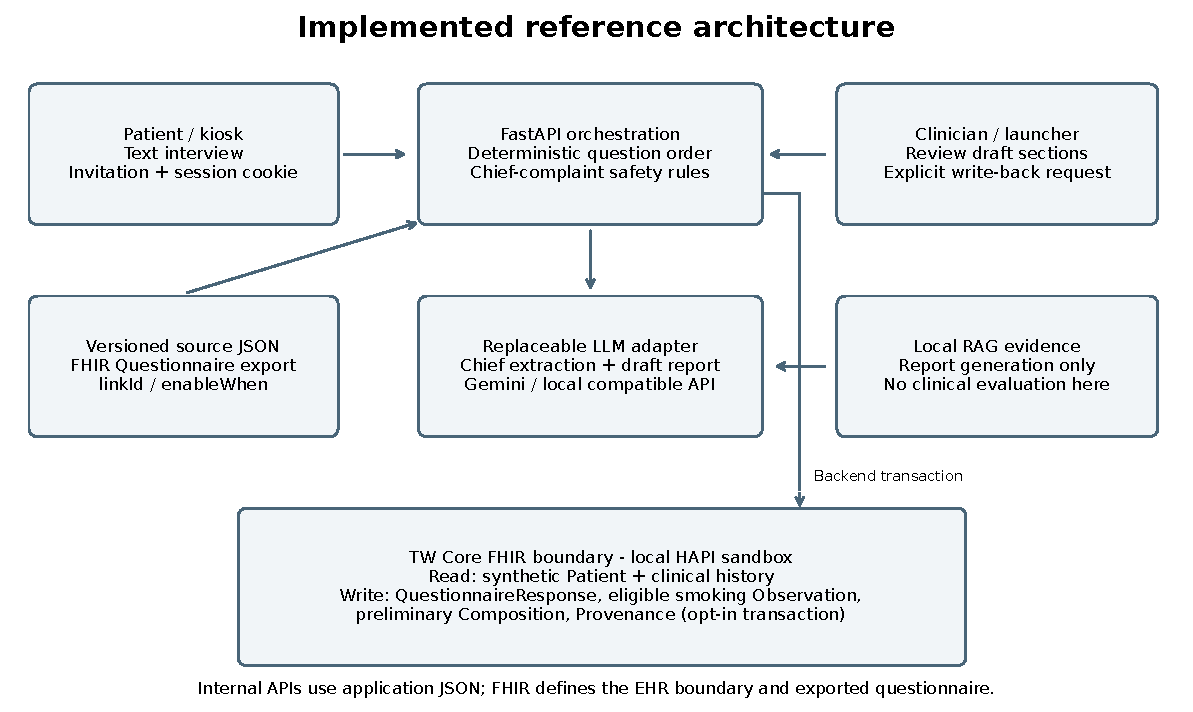
\includegraphics[width=\textwidth]{figures/fig1_architecture.pdf}
\caption{Implemented modules and data boundaries. Source JSON controls the
questionnaire engine; a corresponding FHIR Questionnaire is exported. Internal
APIs use application JSON, while FHIR defines the EHR boundary.}
\label{fig:architecture}
\end{figure}

Question selection is deterministic: the engine asks the next enabled question
and skips EHR-prefilled fields. Rules and evidence-checked model extraction screen
the chief complaint; failed semantic assessment triggers manual handoff. At
routine completion, retrieval supplies evidence for model-generated report
sections and decision-support suggestions. These suggestions are neither
validated diagnoses nor published orders.

\subsection{Questionnaire and write-back contracts}
The encoder maps source fields to stable \texttt{linkId} values, options to coded
answers, and supported conditions to \texttt{enableWhen}. Questionnaire and
QuestionnaireResponse separate form definitions from answers \citep{fhirQuestionnaireR4,sdcIG}.
The canonical version includes a source digest and is pinned in the interview
trace when a route is selected. Write-back rejects a changed canonical version;
older records without a pin use current resolution with an explicit legacy tag.
Application extensions carry source and presentation semantics, so generic FHIR
consumers cannot assume complete runtime equivalence.

Structured write-back is opt-in; Composition-only write-back remains the default.
After simulated clinician confirmation, an authorized request creates the
transaction in Table~\ref{tab:fhir}. Stable references and conditional creation
support retry idempotency. Patient, encounter, institution, and issuer checks
precede persistence. No differential-diagnosis Conditions, ClinicalImpressions,
ServiceRequests, or safety Flags are created.

\begin{table}[t]\centering\small
\caption{Write-back resources and assertion boundaries.}\label{tab:fhir}
\begin{tabular}{lp{8.1cm}}\hline
Resource & Content and boundary \\\hline
QuestionnaireResponse & Ordered answers, source markers, and the pinned canonical reference. \\
Observation & Smoking status only for an explicit mapped patient selection; EHR text is not promoted to a new patient assertion. \\
Composition & Preliminary narrative, confirmed sections, and links to structured answers. \\
Provenance & Patient informant, AI assembly, and simulated clinician-review roles; no actual clinical approval. \\\hline
\end{tabular}
\end{table}

An absent-EHR placeholder is omitted from the response. Free text outside the
option grammar is represented by the existing coded ``other'' option plus its
nested string, retaining both the original text and answer-source marker. This
avoids the validator's incompatible open-choice string/coded-condition exception
without inventing a clinical selection. The original minimal reproduction is
retained. When an answered runtime branch would lose its answer in FHIR,
write-back fails closed with a non-retryable unprocessable-content response;
unanswered branches do not create answers or block writing.

\subsection{Synthetic inputs and model disclosure}
Synthea generated the adult source cohort \citep{syntheaMethod,syntheaSoftware}.
Conversion assigns fictional Taiwanese identifiers and addresses and applies
TW Core profiles \citep{twcoreIG}. Seeds, mappings, dropped elements, and content
hashes are recorded. Taiwan-styled presentation does not establish local disease
representativeness. Input validation is separate from system-output validation.
The \ScenarioCount{} author-drafted scenarios cover chest pain, headache, and
abdominal pain, including expected safety stops and known rule gaps. The planned
benchmark was unavailable. Separate source-level Synthea modules provide
scenario-consistent backgrounds; generated patient records are not manually
rewritten to force agreement.

Mechanical audits check conditions, medications, allergies, and smoking history.
Human approval requires two independent physician decisions against current
script hashes, including patient bindings and expected paths. At generation,
\ValidatedScriptCount{} scripts have those approvals. Model and sampling
settings are disclosed by role in Supplementary Tables~\ref{tab:llmroles}
and~\ref{tab:llmprompts}. Commercial models use remote APIs; local Gemma and
Qwen use Ollama \citep{ollamaSoftware,gemmaThree,qwenTwoFive}.
Requested temperature is distinguished from the transmitted value: the Gemini
adapter omits temperature for the configured newer Gemini models. Provider-effective
sampling and unrecorded historical thinking settings are not inferred from defaults.
Implementation, scenario drafting, orchestration, reference checking, and manuscript
revision used AI assistance; the declarations specify the remaining author review.

\subsection{Verification procedures}
E1 uses the pinned HL7 validator with TW Core and generated questionnaire and
extension definitions \citep{hl7Validator,twcoreIG}. Structural/profile checks use
\texttt{-tx n/a}; they do not establish complete terminology resolution.
The prespecified target is no errors on written resources. Missing outcomes and
validator exceptions are failed verification, reported separately from profile
errors. Round-trip comparison ignores specified server metadata and assigned
identifiers but preserves substantive differences. The independent E1 cohort uses
the same seeded patient selection and fixed short complaints as the earlier run.
A supplemental E1 validates the new E2 outputs without double counting.

The pinned TW Core Provenance binding references participant-type CodeSystem
version 4.0.1, unavailable in the local terminology cache. Explicitly substituting
a different cached version produced binding errors in a diagnostic fixture; we
therefore retained the correct system URI and reported the warnings. Composition
narrative warnings are also retained (Supplementary Table~\ref{tab:warnings}).

E2 runs the patient-facing API through invitation, dialogue, report generation,
simulated clinician confirmation, transaction, and read-back. A distinct local
Qwen model plays the patient using only scenario facts. Invalid constrained
answers receive an explicit unknown fallback, never an expected-answer substitution.
Completion requires successful write-back and an explicit \texttt{completed} or
\texttt{summary\_ready} workflow. This includes successful chief-complaint safety
stops and recovery after a timeout, but excludes manual handoff. We separately
report completion without observed timeout. Timing retains all API write-backs.
Protocol adherence excludes expected red-flag chief stops from comparable paths;
unexpected stops remain failures in the denominator. Traceability uses every
persisted chief-complaint fact, including any missing evidence, and checks its
span against patient utterances. Functional tests compare rule identifiers; they
are not sensitivity or specificity measurements.

E3 changes only module configuration and repeats workflow and FHIR checks.
A complete replacement requires completion without handoff and successful FHIR
verification; successful model invocation alone is insufficient. One-time adapter
implementation is measured separately against base commit \texttt{1b0eb1c}.
Safe session/request identifiers link parser counts, post-validation counts,
schema failures, and bounded-operation timeouts. Candidate-check failures are
not unique rejected facts. Local system and simulated-patient models share GPU
resources. E4 replays captured turns with either fixed-latency mock responses or
real models, using backend v0.18.0 after this fix round and one worker. The
prespecified stop criterion remains request error rate above five percent;
session failure is a separate endpoint. The asynchronous HTTP harness replaces
the planned k6/Locust tool. E5 remains blocked pending exchange-hub access.

Results are descriptive; repetitions are not independent clinical observations.
Tables show actual denominators and median/interquartile summaries. Cost covers
bounded interactive request calls only: background summaries and late calls can
be absent, and every usage record declares incomplete coverage. A successful
recorded call can coexist with an outer operation timeout. Source hashes and
explicit run selection generate all result macros, tables, and figures.

\section{Results}\label{sec:results}

\subsection{Interoperability}
Independent validation of the converted input cohort covers \InputBundles{}
bundles and \InputResources{} resources, with \InputErrors{} errors and
\InputWarnings{} warnings. This combines unchanged outcomes with hash-checked
revalidation of modified bundles and is separate from system-output conformance.

E1 includes \EOneTemplatedSessions{} independent input-cohort sessions and
\EOneScenarioSessions{} E2 sessions. The \EOneResources{} written resources
have \EOneErrors{} errors and \EOneValidatorCrashes{} validator exceptions.
All \EOneQuestionnaireResponses{} QuestionnaireResponses have explicit outcomes,
with \EOneQRErrors{} errors and \EOneQRUnverified{} unverified responses.
The zero-error target is met in both cohorts (Tables~\ref{tab:e1}
and~\ref{tab:e1workflow}). The retained \EOneWarnings{} warnings comprise
\EOneProvenanceWarnings{} Provenance terminology warnings and
\EOneCompositionWarnings{} Composition narrative warnings. The previous QR
verification gap is resolved by faithful nested-text encoding.

\begin{table}[t]\centering
\caption{E1 written-resource validation. Input checks are excluded; exceptions
would count as failed verification.}\label{tab:e1}
\footnotesize\setlength{\tabcolsep}{3pt}
% Generated; edit source results or generator, never these values.
\begin{tabular}{llllll}
\hline
Cohort & Resource & $n$ & With errors & Errors & Warnings \\
\hline
Templated cohort & Composition & 200 & 0 & 0 & 200 \\
Templated cohort & Observation & 197 & 0 & 0 & 0 \\
Templated cohort & Provenance & 200 & 0 & 0 & 800 \\
Templated cohort & QuestionnaireResponse & 200 & 0 & 0 & 0 \\
Scenario cohort & Composition & 150 & 0 & 0 & 150 \\
Scenario cohort & Observation & 100 & 0 & 0 & 0 \\
Scenario cohort & Provenance & 150 & 0 & 0 & 600 \\
Scenario cohort & QuestionnaireResponse & 150 & 0 & 0 & 0 \\
\hline
\end{tabular}

\end{table}
\begin{table}[t]\centering
\caption{E1 workflow and semantic round trip. Read uses all sessions; write uses
attempted writes; read-back uses returned references; round trip uses all captured
submissions, including those without read-back.}\label{tab:e1workflow}
\scriptsize\setlength{\tabcolsep}{3pt}
% Generated; edit source results or generator, never these values.
\begin{tabular}{llllll}
\hline
Cohort & Sessions & Read & Write & Read-back & Round-trip \\
\hline
Templated cohort & 200 & \shortstack{100.0\%\\(200/200)} & \shortstack{100.0\%\\(200/200)} & \shortstack{100.0\%\\(797/797)} & \shortstack{100.0\%\\(797/797)} \\
Scenario cohort & 150 & \shortstack{100.0\%\\(150/150)} & \shortstack{100.0\%\\(150/150)} & \shortstack{100.0\%\\(550/550)} & \shortstack{100.0\%\\(550/550)} \\
\hline
\end{tabular}

\end{table}

\subsection{Workflow and model replacement}
E2 contains \ETwoSessions{} sessions, with \ETwoRepeats{} repetitions per script.
Completion is \ETwoCompletion{}, path agreement is \ETwoProtocol{}, and
fact traceability is \ETwoTraceability{} (Table~\ref{tab:e2}). All
\ETwoChiefStops{} chief stops completed write-back. The
\ETwoInvalidTurns{} invalid simulated-patient turns used explicit unknown
fallbacks. There were \ETwoTimeoutSessions{} timeout-affected sessions;
\ETwoTimeoutStored{} retained a record and \ETwoTimeoutCompleted{} eventually
completed after retry. Completion without observed timeout was
\ETwoTimeoutFreeCompleted{} of \ETwoSessions{}. Table~\ref{tab:e2checks}
reports functional checks and partial usage; independent audit fields remain blank.

\begin{table}[t]\centering
\caption{E2 software workflow outcomes. Percentages show actual numerators and
denominators; path comparison excludes expected chief stops.}\label{tab:e2}
\scriptsize\setlength{\tabcolsep}{2pt}
% Generated; edit source results or generator, never these values.
\begin{tabular}{lllllll}
\hline
Cohort & $n$ & Completion & Path exact & \shortstack{Traceable\\facts} & \shortstack{Turns\\median [Q1,Q3]} & \shortstack{Median seconds\\{}[Q1,Q3]} \\
\hline
Chest pain & 50 & \shortstack{100.0\%\\(50/50)} & \shortstack{100.0\%\\(35/35)} & \shortstack{100.0\%\\(144/144)} & 15.5 [1.0, 17.0] & 35.9 [12.9, 40.3] \\
Headache & 50 & \shortstack{100.0\%\\(50/50)} & \shortstack{100.0\%\\(30/30)} & \shortstack{100.0\%\\(152/152)} & 14.5 [1.0, 15.0] & 33.9 [9.1, 38.3] \\
Abdominal pain & 50 & \shortstack{100.0\%\\(50/50)} & \shortstack{100.0\%\\(35/35)} & \shortstack{100.0\%\\(158/158)} & 13.0 [1.0, 15.0] & 32.7 [13.4, 36.6] \\
Overall & 150 & \shortstack{100.0\%\\(150/150)} & \shortstack{100.0\%\\(100/100)} & \shortstack{100.0\%\\(454/454)} & 15.0 [1.0, 15.0] & 34.6 [12.1, 38.9] \\
\hline
\end{tabular}

\end{table}
\begin{table}[t]\centering
\caption{E2 functional-test pass rates and bounded observed usage. Costs exclude
local hardware and unrecorded calls.}\label{tab:e2checks}
\footnotesize\setlength{\tabcolsep}{4pt}
% Generated; edit source results or generator, never these values.
\begin{tabular}{ll}
\hline
Overall provisional measurement & Observed value \\
\hline
Red-flag functional-test pass rate: exact rules & 83.3\% (50/60) \\
Red-flag functional-test pass rate: acceptable rules & 83.3\% (50/60) \\
Other-script functional-test pass rate: no unexpected rules & 100.0\% (90/90) \\
Sessions with documented rule-coverage gaps & 10 \\
Sessions with recorded model usage & 150 \\
System input tokens/session, median & 17,014 \\
System output tokens/session, median & 1,776 \\
Simulated-patient tokens/session, median & 17,522 \\
Observed API cost/session, median USD & 0.0177 \\
Sessions contributing cost estimates & 110 \\
Invalid simulated-patient turns & 48 \\
\hline
\end{tabular}

\end{table}

The \EThreeConfigurations{} E3 configurations used identical executable
fingerprints throughout. One-time LLM adapter work added \AdapterAdded{} and
removed \AdapterRemoved{} lines relative to the base commit, restricted to the
adapter-related files; subsequent configuration swaps required no code changes.
The commercial alternate met eventual-completion and FHIR criteria, although
\EThreeAlternateTimeoutSessions{} sessions recovered after timeouts. The local Gemma
replacement did not: completion without handoff was \EThreeLocalCompletion{},
despite successful FHIR checks (Table~\ref{tab:e3}). Its unexpected stops remain
path failures; only expected stops are excluded from that denominator.

\begin{table}[t]\centering
\caption{E3 model replacement. Code changes exclude one-time adapter work.
Completion excludes handoff. Costs are partial API-charge estimates; local zero
excludes hardware and omitted calls.}\label{tab:e3}
\scriptsize\setlength{\tabcolsep}{1.8pt}
% Generated; edit source results or generator, never these values.
\begin{tabular}{llllllll}
\hline
Configuration & \shortstack{Code\\lines} & Completion & Path exact & Facts & Errors & \shortstack{Median\\seconds} & USD/session* \\
\hline
\shortstack{Default\\Gemini} & 0 & \shortstack{100.0\%\\(30/30)} & \shortstack{100.0\%\\(20/20)} & \shortstack{100.0\%\\(91/91)} & 0 & 40.0 & \shortstack{0.0192\\($n$=22)} \\
\shortstack{Alternate\\Gemini} & 0 & \shortstack{100.0\%\\(30/30)} & \shortstack{100.0\%\\(20/20)} & \shortstack{100.0\%\\(114/114)} & 0 & 34.5 & \shortstack{0.0096\\($n$=22)} \\
\shortstack{Local\\Gemma 3} & 0 & \shortstack{93.3\%\\(28/30)} & \shortstack{90.9\%\\(20/22)} & \shortstack{100.0\%\\(6/6)} & 0 & 205.7 & \shortstack{0.0000\\($n$=20)} \\
\hline
\end{tabular}

\end{table}

Persisted facts were \EThreeDefaultFacts{} for the default,
\EThreeAlternateFacts{} for the commercial alternate, and \EThreeLocalFacts{}
for Gemma. Gemma's \EThreeLocalChiefCalls{} extraction calls produced
\EThreeLocalParsedSymptoms{} parsed symptom candidates but retained only
\EThreeLocalRetainedSymptoms{}; findings were absent before and after validation.
No local schema/parser failures were observed (Table~\ref{tab:e3diagnostics}).
AP-07 and HA-08 did not stop at chief screening; HA-08 retained only a headache
fact. AP-03 and AP-04 entered manual handoff after chief-assessment timeouts;
late worker completion did not reverse these outcomes. Gemma's
\EThreeLocalTimeoutSessions{} timeout-affected sessions all retained records,
but only \EThreeLocalTimeoutCompleted{} completed without handoff.
All \EThreeLocalUsageCalls{} captured usage calls reported \texttt{ok}; this
bounded lower-level status did not describe the timed-out outer operations.
The earlier excluded run lacks pre-validation diagnostics, preventing precise
retrospective attribution of its low extraction yield.

\subsection{Local load}
Mock load at concurrency \ELoadHundredConcurrency{} had p95 per-turn latency of
\ELoadHundredPninetyfiveSeconds{} seconds. At \ELoadLastConcurrency{},
\ELoadLastCompleted{} of \ELoadLastSessions{} sessions completed; request error
was \ELoadLastRequestError{} and session failure \ELoadLastSessionFailure{}.
The request-error stopping threshold was not crossed despite high session failure.
The lower p95 at the highest level is subject to survivorship: sessions failing
early contribute no later-turn latency. It does not establish faster successful
workflows (Fig.~\ref{fig:load}; Supplementary Table~\ref{tab:e4levels}).
Real mode completed \ERealCompleted{} of \ERealSessions{} sessions at concurrency
\ERealConcurrency{}. Both modes replay the selected E2 source but use different
load levels and patient pools; these are local descriptive measurements.
National peak demand remains \texttt{TODO\_PEAK\_DEMAND}. E5 has no measured result.

\begin{figure}[t]\centering
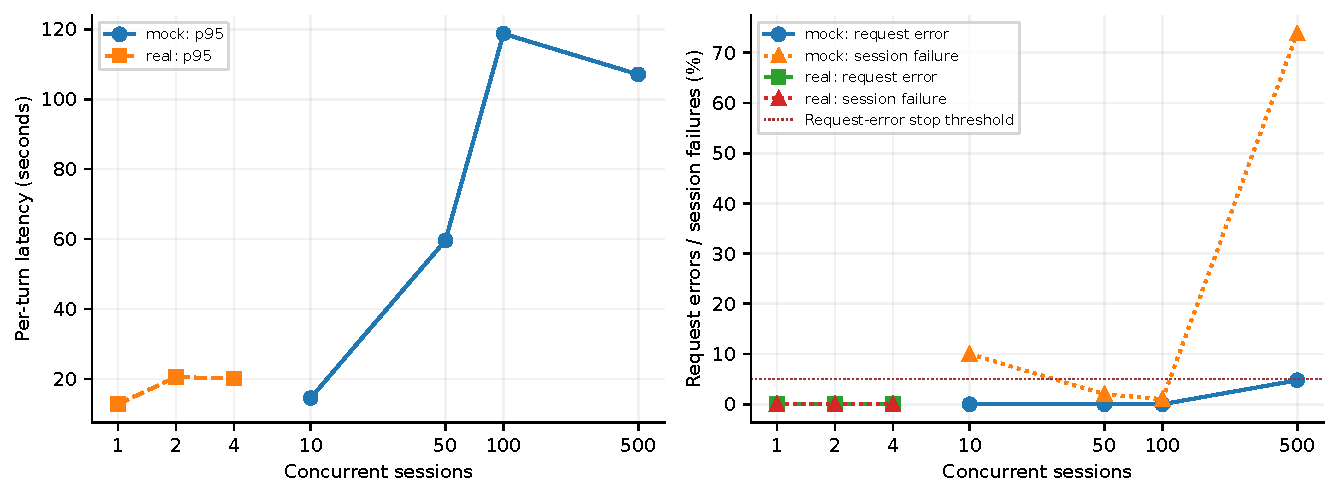
\includegraphics[width=\textwidth]{figures/fig_e4_load.pdf}
\caption{Local synthetic load on the fixed backend. The dotted line is the
request-error stop threshold, not a session-failure threshold. Per-turn latency
includes observed HTTP attempts; early failures truncate later measurements.}
\label{fig:load}
\end{figure}

\section{Discussion}\label{sec:discussion}
Verification distinguishes data fidelity from successful transport. Nested
``other'' encoding preserved unrecognized EHR text while resolving QR validation
exceptions. Version pinning and answered-branch guards make incompatible changes
explicit. These contracts are narrower than a universal FHIR-native internal bus:
source JSON still controls interviews and extensions carry application semantics.

Model configurability likewise does not guarantee equivalent behavior. Gemma's
low fact yield arose with nonempty symptom candidates that disappeared during
local code/evidence validation, absent findings, and separate operation timeouts.
The diagnostics do not retain raw candidate JSON, so they cannot allocate each
removed candidate to incorrect codes, unsupported evidence, or deduplication.
A traceability percentage over a small surviving set cannot establish coverage.
The failed completion criterion and missed scripted stops preclude a claim of
complete local-model interchangeability under the tested settings.

\subsection{Limitations and clinical review needs}
This is software verification, not evidence of clinical safety, diagnostic
performance, utility, or deployment readiness. Scenarios await physician review;
synthetic demographics are not representative, the patient simulator may
hallucinate, and evidence spans do not validate clinical interpretation. Only
chief-complaint screening runs in the default engine. Later questionnaire
selections such as diaphoresis, syncope, fever with neck stiffness, unclear speech,
or abdominal rigidity/rebound pain do not trigger renewed screening.
Rules omit suspected pulmonary embolism (CP-09), abdominal aortic aneurysm without
syncope (AP-10), and sustained exertional pressure without diaphoresis or syncope.
The structured ectopic-pregnancy combination depends on prefilled pregnancy risk,
although a separate raw rule can match explicit pregnancy and bleeding. The raw
negation window treats single negation characters broadly: a phrase describing
limb weakness followed by unclear speech can suppress the neurologic match.
These code-level gaps require qualified clinical review; no rules were changed.

Cost telemetry is incomplete. Local models share GPU capacity, commercial aliases
may change, and recorded versions cannot make remote inference deterministic.
The sandbox does not establish production authorization, tenant isolation,
browser SMART integration, or national capacity. Independent transcript and
fact audits, terminology review, institutional governance, and exchange-hub access
remain necessary before further acceptance.

\section{Conclusion}\label{sec:conclusion}
The fixed implementation meets the written-resource verification target and
supports inspectable questionnaire, provenance, and write-back contracts.
Model replacement and load results expose operational limits that successful
FHIR transfer alone would conceal. Clinical evaluation remains separate.

\backmatter
\bmhead{Supplementary information}
The repository preserves immutable runs, source hashes, scripts, reviewer packets,
and analysis code. The independent E1 cohort rotates fixed brief complaints across
seeded patients. The harness composes option answers as the kiosk does, records
invalid attempts, and uses exact unknown-option matching; an earlier substring
fallback was excluded because it could select a symptom-containing option.
Run-created resources are captured and removed before patient reuse. Shared
patients are serialized within a run, and experiments run sequentially after
baseline checks. No current chest-pain scenario has human approval, so a
clinician-approved walkthrough remains unavailable.

Table~\ref{tab:e3diagnostics} separates chief stops, extraction yield, and timeouts;
Table~\ref{tab:gemmasessions} gives each local-model session. Timeout logs and
bounded-operation events can describe the same incident and are not added.
Parser/shape failures are local observations, not proof of remote schema enforcement.

\begin{table}[p]\centering
\caption{E3 extraction and operation diagnostics. Expected chief stops alone are
excluded from path comparison; unexpected stops remain failures.}\label{tab:e3diagnostics}
\scriptsize\setlength{\tabcolsep}{2pt}
% Generated; edit source results or generator, never these values.
\begin{tabular}{p{0.44\linewidth}ccc}
\hline
Observed measurement & \shortstack{Default\\Gemini} & \shortstack{Alternate\\Gemini} & \shortstack{Local\\Gemma 3} \\
\hline
Sessions & 30 & 30 & 30 \\
Persisted facts & 91 & 114 & 6 \\
Chief stops (all) & 10 & 10 & 10 \\
Chief stops with eventual completion & 10 & 10 & 8 \\
Unexpected chief stops & 0 & 0 & 2 \\
Eventual completion (no handoff) & \shortstack{100.0\%\\(30/30)} & \shortstack{100.0\%\\(30/30)} & \shortstack{93.3\%\\(28/30)} \\
Manual handoffs & 0 & 0 & 2 \\
Expected chief stops excluded from path test & 10 & 10 & 8 \\
Red-flag functional-test pass rate & \shortstack{83.3\%\\(10/12)} & \shortstack{83.3\%\\(10/12)} & \shortstack{66.7\%\\(8/12)} \\
Sessions with observed timeout & 0 & 2 & 12 \\
Timeout sessions: stored record & 0 & 2 & 12 \\
Timeout sessions: API write-back & 0 & 2 & 12 \\
Timeout sessions: eventual completion & 0 & 2 & 10 \\
Completion without observed timeout & 30 & 28 & 18 \\
Bounded-operation timeout events & 0 & 2 & 12 \\
Timeout log events (not additive) & 0 & 2 & 10 \\
Observed chief extraction calls & 22 & 22 & 22 \\
Local parser/shape failures & 0 & 0 & 0 \\
Symptoms: parsed to post-validation & 22 $\to$ 22 & 28 $\to$ 22 & 108 $\to$ 6 \\
Findings: parsed to post-validation & 52 $\to$ 51 & 53 $\to$ 53 & 0 $\to$ 0 \\
Assessments: parsed to post-validation & 22 $\to$ 22 & 28 $\to$ 22 & 22 $\to$ 0 \\
Questionnaire answers: parsed to post-validation & 45 $\to$ 52 & 67 $\to$ 70 & 0 $\to$ 20 \\
\hline
\end{tabular}

\end{table}
\begin{table}[p]\centering
\caption{Gemma session diagnostics. Symptoms show parsed to retained candidates;
``--'' means no extractor call. Handoff* includes worker events occurring after
session completion; these do not undo handoff. Empty usage is not zero consumption.}
\label{tab:gemmasessions}
\scriptsize\setlength{\tabcolsep}{3pt}
% Generated; edit source results or generator, never these values.
\begin{tabular}{llllllll}
\hline
Script & Workflow & Facts & \shortstack{Symptoms\\parsed $\to$\\retained} & \shortstack{Findings\\parsed $\to$\\retained} & \shortstack{Schema\\failures} & \shortstack{Timeout\\(events)} & \shortstack{Usage\\status/calls} \\
\hline
AP-01 & Completed & 0 & 3 $\to$ 0 & 0 $\to$ 0 & 0 & RAG (1) & ok/16 \\
AP-02 & Completed & 0 & 3 $\to$ 0 & 0 $\to$ 0 & 0 & RAG (1) & ok/15 \\
AP-03 & Handoff* & 0 & 3 $\to$ 0 & 0 $\to$ 0 & 0 & Chief (1) & Empty/0 \\
AP-04 & Handoff* & 0 & 3 $\to$ 0 & 0 $\to$ 0 & 0 & Chief (1) & Empty/0 \\
AP-05 & Completed & 0 & 3 $\to$ 0 & 0 $\to$ 0 & 0 & None & ok/16 \\
AP-06 & Completed & 0 & 3 $\to$ 0 & 0 $\to$ 0 & 0 & None & ok/16 \\
AP-07 & Completed & 0 & 3 $\to$ 0 & 0 $\to$ 0 & 0 & RAG (1) & ok/15 \\
AP-08 & Chief stop & 0 & -- $\to$ -- & -- $\to$ -- & 0 & None & Empty/0 \\
AP-09 & Chief stop & 0 & -- $\to$ -- & -- $\to$ -- & 0 & None & Empty/0 \\
AP-10 & Completed & 0 & 3 $\to$ 0 & 0 $\to$ 0 & 0 & RAG (1) & ok/15 \\
CP-01 & Completed & 0 & 11 $\to$ 0 & 0 $\to$ 0 & 0 & RAG (1) & ok/15 \\
CP-02 & Completed & 0 & 11 $\to$ 0 & 0 $\to$ 0 & 0 & None & ok/16 \\
CP-03 & Completed & 0 & 11 $\to$ 0 & 0 $\to$ 0 & 0 & RAG (1) & ok/16 \\
CP-04 & Completed & 0 & 11 $\to$ 0 & 0 $\to$ 0 & 0 & RAG (1) & ok/15 \\
CP-05 & Completed & 0 & 11 $\to$ 0 & 0 $\to$ 0 & 0 & None & ok/16 \\
CP-06 & Completed & 0 & 11 $\to$ 0 & 0 $\to$ 0 & 0 & None & ok/16 \\
CP-07 & Chief stop & 0 & -- $\to$ -- & -- $\to$ -- & 0 & None & Empty/0 \\
CP-08 & Chief stop & 0 & -- $\to$ -- & -- $\to$ -- & 0 & None & Empty/0 \\
CP-09 & Completed & 0 & 11 $\to$ 0 & 0 $\to$ 0 & 0 & RAG (1) & ok/14 \\
CP-10 & Chief stop & 0 & -- $\to$ -- & -- $\to$ -- & 0 & None & Empty/0 \\
HA-01 & Completed & 1 & 1 $\to$ 1 & 0 $\to$ 0 & 0 & None & ok/16 \\
HA-02 & Completed & 1 & 1 $\to$ 1 & 0 $\to$ 0 & 0 & None & ok/16 \\
HA-03 & Completed & 1 & 1 $\to$ 1 & 0 $\to$ 0 & 0 & None & ok/16 \\
HA-04 & Completed & 1 & 1 $\to$ 1 & 0 $\to$ 0 & 0 & RAG (1) & ok/15 \\
HA-05 & Completed & 1 & 1 $\to$ 1 & 0 $\to$ 0 & 0 & RAG (1) & ok/15 \\
HA-06 & Completed & 0 & 1 $\to$ 0 & 0 $\to$ 0 & 0 & None & ok/16 \\
HA-07 & Chief stop & 0 & -- $\to$ -- & -- $\to$ -- & 0 & None & Empty/0 \\
HA-08 & Completed & 1 & 1 $\to$ 1 & 0 $\to$ 0 & 0 & None & ok/16 \\
HA-09 & Chief stop & 0 & -- $\to$ -- & -- $\to$ -- & 0 & None & Empty/0 \\
HA-10 & Chief stop & 0 & -- $\to$ -- & -- $\to$ -- & 0 & None & Empty/0 \\
\hline
\end{tabular}

\end{table}
\begin{table}[p]\centering
\caption{Every measured load level. Latency is per observed turn; completion and
request errors have different denominators.}\label{tab:e4levels}
\scriptsize\setlength{\tabcolsep}{3pt}
% Generated; edit source results or generator, never these values.
\begin{tabular}{llllll}
\hline
Mode & Concurrency & Completed & Request error & Session failure & Turn p95 (s) \\
\hline
Mock & 10 & 9/10 & 0.00\% & 10.00\% & 1.5 \\
Mock & 50 & 49/50 & 0.00\% & 2.00\% & 65.0 \\
Mock & 100 & 99/100 & 0.00\% & 1.00\% & 121.3 \\
Mock & 500 & 130/500 & 4.71\% & 74.00\% & 112.8 \\
Real & 1 & 1/1 & 0.00\% & 0.00\% & 13.7 \\
Real & 2 & 2/2 & 0.00\% & 0.00\% & 20.5 \\
Real & 4 & 4/4 & 0.00\% & 0.00\% & 21.3 \\
\hline
\end{tabular}

\end{table}
\begin{table}[p]\centering
\caption{Retained E1 warnings across both written-resource cohorts.}\label{tab:warnings}
\scriptsize\setlength{\tabcolsep}{3pt}
% Generated; edit source results or generator, never these values.
\begin{tabular}{rp{11cm}}
\hline
Count & Warning \\
\hline
1,400 & A definition for CodeSystem 'http:/\allowbreak{}/\allowbreak{}terminology.hl7.org/\allowbreak{}CodeSystem/\allowbreak{}provenance-\allowbreak{}participant-\allowbreak{}type' version '4.0.1' could not be found, so the code cannot be validated. Valid versions: 0.1.0, 1.1.0 or 2.0 \\
350 & Constraint failed: dom-\allowbreak{}6: 'A resource should have narrative for robust management' (defined in http:/\allowbreak{}/\allowbreak{}hl7.org/\allowbreak{}fhir/\allowbreak{}StructureDefinition/\allowbreak{}DomainResource) (Best Practice Recommendation) \\
\hline
\end{tabular}

\end{table}
\begin{table}[p]\centering
\caption{E2 restricted to currently physician-approved script hashes. No approved
scripts are available; absent results are not zero-valued successes.}\label{tab:validated}
\scriptsize\setlength{\tabcolsep}{2pt}
% Generated; edit source results or generator, never these values.
\begin{tabular}{lllllll}
\hline
Cohort & $n$ & Completion & Path exact & \shortstack{Traceable\\facts} & \shortstack{Turns\\median [Q1,Q3]} & \shortstack{Median seconds\\{}[Q1,Q3]} \\
\hline
Chest pain & 0 & -- & -- & -- & -- & -- \\
Headache & 0 & -- & -- & -- & -- & -- \\
Abdominal pain & 0 & -- & -- & -- & -- & -- \\
Overall & 0 & -- & -- & -- & -- & -- \\
\hline
\end{tabular}

\end{table}

\begin{table}[p]\centering
\caption{Models by executed configuration and role. Version strings are pinned
metadata; dates are UTC. A configured role need not run in every session.}
\label{tab:llmroles}\scriptsize\setlength{\tabcolsep}{3pt}
% Generated; edit source results or generator, never these values.
\begin{tabular}{p{0.21\linewidth}p{0.17\linewidth}p{0.33\linewidth}p{0.17\linewidth}}
\hline
Configuration / role & Provider / access & Model ID / recorded version & Run dates (UTC) \\
\hline
Default Gemini: Chief extraction & Gemini, remote API & gemini-\allowbreak{}3.\allowbreak{}6-\allowbreak{}flash\newline 3.\allowbreak{}6-\allowbreak{}flash-\allowbreak{}07-\allowbreak{}2026 & 2026-\allowbreak{}10-\allowbreak{}13 \\
Default Gemini: Summary extraction & Gemini, remote API & gemini-\allowbreak{}3.\allowbreak{}5-\allowbreak{}flash-\allowbreak{}lite\newline 3.\allowbreak{}5-\allowbreak{}flash-\allowbreak{}lite-\allowbreak{}07-\allowbreak{}2026 & 2026-\allowbreak{}10-\allowbreak{}13 \\
Default Gemini: Summary reasoning & Gemini, remote API & gemini-\allowbreak{}3.\allowbreak{}6-\allowbreak{}flash\newline 3.\allowbreak{}6-\allowbreak{}flash-\allowbreak{}07-\allowbreak{}2026 & 2026-\allowbreak{}10-\allowbreak{}13 \\
Default Gemini: RAG translation & Gemini, remote API & gemini-\allowbreak{}3.\allowbreak{}5-\allowbreak{}flash-\allowbreak{}lite\newline 3.\allowbreak{}5-\allowbreak{}flash-\allowbreak{}lite-\allowbreak{}07-\allowbreak{}2026 & 2026-\allowbreak{}10-\allowbreak{}13 \\
Default Gemini: Simulated patient & Ollama, local API & qwen2.\allowbreak{}5:\allowbreak{}7b-\allowbreak{}instruct\newline 845dbda0\allowbreak{}ea48ed74\allowbreak{}9caafd9e\allowbreak{}6037047a\allowbreak{}a19acfcf\allowbreak{}d82e704d\allowbreak{}7ca97d63\allowbreak{}1a0b697e & 2026-\allowbreak{}10-\allowbreak{}13 \\
Alternate Gemini: Chief extraction & Gemini, remote API & gemini-\allowbreak{}2.\allowbreak{}5-\allowbreak{}flash\newline 001 & 2026-\allowbreak{}10-\allowbreak{}13 \\
Alternate Gemini: Summary extraction & Gemini, remote API & gemini-\allowbreak{}2.\allowbreak{}5-\allowbreak{}flash\newline 001 & 2026-\allowbreak{}10-\allowbreak{}13 \\
Alternate Gemini: Summary reasoning & Gemini, remote API & gemini-\allowbreak{}2.\allowbreak{}5-\allowbreak{}flash\newline 001 & 2026-\allowbreak{}10-\allowbreak{}13 \\
Alternate Gemini: RAG translation & Gemini, remote API & gemini-\allowbreak{}3.\allowbreak{}5-\allowbreak{}flash-\allowbreak{}lite\newline 3.\allowbreak{}5-\allowbreak{}flash-\allowbreak{}lite-\allowbreak{}07-\allowbreak{}2026 & 2026-\allowbreak{}10-\allowbreak{}13 \\
Alternate Gemini: Simulated patient & Ollama, local API & qwen2.\allowbreak{}5:\allowbreak{}7b-\allowbreak{}instruct\newline 845dbda0\allowbreak{}ea48ed74\allowbreak{}9caafd9e\allowbreak{}6037047a\allowbreak{}a19acfcf\allowbreak{}d82e704d\allowbreak{}7ca97d63\allowbreak{}1a0b697e & 2026-\allowbreak{}10-\allowbreak{}13 \\
Local Gemma: Chief extraction & Ollama, local API & gemma3:\allowbreak{}12b\newline b92b2185\allowbreak{}82c521ba\allowbreak{}287f38f1\allowbreak{}d6057dcd\allowbreak{}3c6cbff0\allowbreak{}36f13cac\allowbreak{}97b5d861\allowbreak{}f5e58ec3 & 2026-\allowbreak{}10-\allowbreak{}13 \\
Local Gemma: Summary extraction & Ollama, local API & gemma3:\allowbreak{}12b\newline b92b2185\allowbreak{}82c521ba\allowbreak{}287f38f1\allowbreak{}d6057dcd\allowbreak{}3c6cbff0\allowbreak{}36f13cac\allowbreak{}97b5d861\allowbreak{}f5e58ec3 & 2026-\allowbreak{}10-\allowbreak{}13 \\
Local Gemma: Summary reasoning & Ollama, local API & gemma3:\allowbreak{}12b\newline b92b2185\allowbreak{}82c521ba\allowbreak{}287f38f1\allowbreak{}d6057dcd\allowbreak{}3c6cbff0\allowbreak{}36f13cac\allowbreak{}97b5d861\allowbreak{}f5e58ec3 & 2026-\allowbreak{}10-\allowbreak{}13 \\
Local Gemma: RAG translation & Ollama, local API & gemma3:\allowbreak{}12b\newline b92b2185\allowbreak{}82c521ba\allowbreak{}287f38f1\allowbreak{}d6057dcd\allowbreak{}3c6cbff0\allowbreak{}36f13cac\allowbreak{}97b5d861\allowbreak{}f5e58ec3 & 2026-\allowbreak{}10-\allowbreak{}13 \\
Local Gemma: Simulated patient & Ollama, local API & qwen2.\allowbreak{}5:\allowbreak{}7b-\allowbreak{}instruct\newline 845dbda0\allowbreak{}ea48ed74\allowbreak{}9caafd9e\allowbreak{}6037047a\allowbreak{}a19acfcf\allowbreak{}d82e704d\allowbreak{}7ca97d63\allowbreak{}1a0b697e & 2026-\allowbreak{}10-\allowbreak{}13 \\
\hline
\end{tabular}

\end{table}
\begin{table}[p]\centering
\caption{Default Gemini sampling by role. Requested values are distinguished
from values sent by the adapter; provider-effective defaults were not observed.}
\label{tab:llmdefault}\scriptsize\setlength{\tabcolsep}{3pt}
% Generated; edit source results or generator, never these values.
\begin{tabular}{p{0.15\linewidth}p{0.16\linewidth}p{0.12\linewidth}p{0.45\linewidth}}
\hline
Role & Temperature: requested / sent & Seed & Token budget / thinking \\
\hline
Chief extraction & 0 / omitted & not set & 4096. Visible-answer budget; final request limit not recorded (thinking headroom may apply). Thinking: not recorded. \\
Summary extraction & 0.2 / omitted & not set & chief complaint: 240; present illness: 500; past history: 400; drug history: 400; drug allergy history: 300; personal history: 450; family history: 400. Visible-answer budget; final request limit not recorded (thinking headroom may apply). Thinking: not recorded. \\
Summary reasoning & 0.2 / omitted & not set & differential diagnoses: 900; must not miss: 1200; physical examination: 900; laboratory: 1200; imaging: 1200. Visible-answer budget; final request limit not recorded (thinking headroom may apply). Thinking: not recorded. \\
RAG translation & 0 / omitted & not set & 700. Visible-answer budget; final request limit not recorded (thinking headroom may apply). Thinking: not recorded. \\
Simulated patient & 0.0 / 0.0 & 20261013 & 400. Sent unchanged. \\
\hline
\end{tabular}

\end{table}
\begin{table}[p]\centering
\caption{Alternate Gemini sampling by role. Unrecorded historical thinking
settings and final request limits are explicitly unavailable.}
\label{tab:llmalternate}\scriptsize\setlength{\tabcolsep}{3pt}
% Generated; edit source results or generator, never these values.
\begin{tabular}{p{0.15\linewidth}p{0.16\linewidth}p{0.12\linewidth}p{0.45\linewidth}}
\hline
Role & Temperature: requested / sent & Seed & Token budget / thinking \\
\hline
Chief extraction & 0 / 0 & not set & 4096. Visible-answer budget; final request limit not recorded (thinking headroom may apply). Thinking: not recorded. \\
Summary extraction & 0.2 / 0.2 & not set & chief complaint: 240; present illness: 500; past history: 400; drug history: 400; drug allergy history: 300; personal history: 450; family history: 400. Visible-answer budget; final request limit not recorded (thinking headroom may apply). Thinking: not recorded. \\
Summary reasoning & 0.2 / 0.2 & not set & differential diagnoses: 900; must not miss: 1200; physical examination: 900; laboratory: 1200; imaging: 1200. Visible-answer budget; final request limit not recorded (thinking headroom may apply). Thinking: not recorded. \\
RAG translation & 0 / omitted & not set & 700. Visible-answer budget; final request limit not recorded (thinking headroom may apply). Thinking: not recorded. \\
Simulated patient & 0.0 / 0.0 & 20261013 & 400. Sent unchanged. \\
\hline
\end{tabular}

\end{table}
\begin{table}[p]\centering
\caption{Local Gemma system and Qwen simulated-patient sampling by role. Local
API access does not imply zero hardware cost.}
\label{tab:llmlocal}\scriptsize\setlength{\tabcolsep}{3pt}
% Generated; edit source results or generator, never these values.
\begin{tabular}{p{0.15\linewidth}p{0.16\linewidth}p{0.12\linewidth}p{0.45\linewidth}}
\hline
Role & Temperature: requested / sent & Seed & Token budget / thinking \\
\hline
Chief extraction & 0 / 0 & not set & 4096. Sent unchanged. \\
Summary extraction & 0.2 / 0.2 & not set & chief complaint: 240; present illness: 500; past history: 400; drug history: 400; drug allergy history: 300; personal history: 450; family history: 400. Sent unchanged. \\
Summary reasoning & 0.2 / 0.2 & not set & differential diagnoses: 900; must not miss: 1200; physical examination: 900; laboratory: 1200; imaging: 1200. Sent unchanged. \\
RAG translation & 0 / 0 & not set & 700. Sent unchanged. \\
Simulated patient & 0.0 / 0.0 & 20261013 & 400. Sent unchanged. \\
\hline
\end{tabular}

\end{table}
\begin{table}[p]\centering
\caption{Prompt source files and planned human QA by role. Source hashes are in
the disclosure artifact. Automated checks and simulated confirmation do not replace
pending human review.}\label{tab:llmprompts}
\scriptsize\setlength{\tabcolsep}{3pt}
% Generated; edit source results or generator, never these values.
\begin{tabular}{p{0.18\linewidth}p{0.46\linewidth}p{0.24\linewidth}}
\hline
Role & Prompt files (hashes in disclosure JSON) & Human QA status \\
\hline
Chief extraction & backend/\allowbreak{}amie/\allowbreak{}chief\_\allowbreak{}complaint.\allowbreak{}py\newline backend/\allowbreak{}amie/\allowbreak{}chief\_\allowbreak{}complaint\_\allowbreak{}schema.\allowbreak{}py & Pending: clinical scenario review and 10\% fact audit; confirmation simulated. \\
Summary extraction & backend/\allowbreak{}app/\allowbreak{}prompts/\allowbreak{}questionnaire\_\allowbreak{}summary.\allowbreak{}py\newline backend/\allowbreak{}app/\allowbreak{}prompts/\allowbreak{}common.\allowbreak{}py & Pending: clinical scenario review and 10\% fact audit; confirmation simulated. \\
Summary reasoning & backend/\allowbreak{}app/\allowbreak{}prompts/\allowbreak{}questionnaire\_\allowbreak{}summary.\allowbreak{}py\newline backend/\allowbreak{}app/\allowbreak{}prompts/\allowbreak{}common.\allowbreak{}py & Pending: clinical scenario review and 10\% fact audit; confirmation simulated. \\
RAG translation & backend/\allowbreak{}knowledge/\allowbreak{}translation.\allowbreak{}py & Pending: clinical scenario review and 10\% fact audit; confirmation simulated. \\
Simulated patient & experiments/\allowbreak{}prompts/\allowbreak{}patient\_\allowbreak{}agent\_\allowbreak{}v1.\allowbreak{}md & Pending: clinical scenario review and 15\% transcript audit. \\
\hline
\end{tabular}

\end{table}

\begin{table}[p]\centering
\caption{Principal pinned software versions. Full digests accompany manifests.}
\label{tab:versions}\small
% Generated; edit source results or generator, never these values.
\begin{tabular}{ll}
\hline
Component & Pinned version \\
\hline
Synthea & v4.0.0 \\
FHIR & 4.0.1 \\
HAPI image & hapiproject/hapi:v8.8.0-1 \\
TW Core IG & 1.0.0 \\
HL7 validator & 6.10.4 \\
Python & 3.12.15 \\
Node & v22.23.2 \\
Ollama & 0.32.6 \\
default extraction & gemini-3.6-flash \\
default summary extraction & gemini-3.5-flash-lite \\
default summary reasoning & gemini-3.6-flash \\
swap a & gemini-2.5-flash \\
swap b & gemma3:12b \\
patient simulator model & qwen2.5:7b-instruct \\
\hline
\end{tabular}

\end{table}

\bmhead{Acknowledgements}
Author confirmation of acknowledgements and institutional wording is pending.

\section*{Declarations}
\textbf{Funding, competing interests, and contributions.} Authors must supply and
verify these statements and final approval.\par
\textbf{Ethics and consent.} Only synthetic data were used. Authors must confirm
the applicable institutional determination; no ethics approval is asserted.\par
\textbf{Data and code availability.} Scripts, derived summaries, and generators
are in the project repository. Large raw artifacts are regenerable and excluded
from source control. An archival identifier and access statement require author
confirmation.\par
\textbf{AI assistance.} Claude Code and Codex assisted code and scenario drafting,
experiment orchestration, source checking, and manuscript drafting and revision.
Recorded model identifiers, dates, and unavailable settings are disclosed in the
repository. Authors must verify citations, review technical and clinical content,
and approve the final text; scenario approvals and independent audits remain pending.

\bibliography{sn-bibliography}

\end{document}
